\documentclass{article}

%%% SOME USEFUL PACKAGES %%%
\usepackage[english]{babel} % hyphenation
\usepackage[margin=1.5cm]{geometry} % margins
\usepackage{graphicx} % support for graphics
\usepackage{amsmath} % support for math­e­mat­i­cal typesetting
\usepackage{amssymb} % math­e­mat­i­cal symbols
\usepackage{color} % support for colors
\usepackage{mathtools} % more math­e­mat­i­cal type­set­ting
\usepackage{amsthm} % for defining theorem-like environments
\usepackage{enumerate} % change appearance of numbered lists
\usepackage{framed} % textboxes
\usepackage[format=plain,labelfont=bf,up]{caption} % cus­tomise cap­tions for fig­ures and ta­bles
\usepackage[colorlinks=true,linkcolor=black,urlcolor=blue,linktoc=all, citecolor=black]{hyperref} % hyperlinks
\usepackage{setspace}
\usepackage{verbatim}

%%% CUSTOM COMMANDS %%%
\def\ci{\perp\!\!\!\perp} % statistical independence symbol
\newcommand{\ind}{1\hspace{-2.1mm}{1}} % indicator function
\newcommand{\rl}{\mathbb{R}} % real numbers
\newcommand{\ex}[1]{\mathbb{E} \left\{ #1 \right\}} % expectation operator
\newcommand{\pr}[1]{\mathbb{P} \left\{ #1 \right\}} % probability
\newcommand{\var}[1]{\mathbb{V}\text{ar} \left\{ #1 \right\}} % variance
\newcommand{\cov}[1]{\mathbb{C}{ov} \left\{ #1 \right\}} % covariance
\newcommand{\corr}[1]{\mathbb{C}{orr} \left\{ #1 \right\}} % correlation

\begin{document}
	\title{OSM Lab 2017: Perturbation Methods Pset }
	\author{Wei Han Chia}
	\date{Due: 28 July 2017}
	\maketitle
	
	\section*{Perturbation Methods}
	
	\subsection*{Exercise 1}
	We suppress the input notation for simplification. Note that for our cubic approximation, we require $x_{uuu}(u_{0})$, and so we need to differentiate (5) again with respect to $u$.
	
	\begin{align*}
	&F_{xx} x_u^2 + F_{xu} x_u + F_{x} x_{uu} + F_{xu} x_u + F_{uu} = 0 \\
	&\text{Taking derivative w.r.t $u$} \\
	&F_{xxx} x_u^3 + F_{xxu}x_u^2 + 2 F_{xx} x_u x_{uu} +  \\
	&F_{xux} x_u^2 + F_{xuu} x_u + F_{xu} x_{uu} + \\
	&F_{xx} x_{uu} x_{u} + F_{xu} x_{uu} + F_{x} x_{uuu} + \\
	&F_{xux} x_{u}^2 + F_{xuu} x_u + F_{xu} x_{uu} + \\
	&F_{uux} x_{u} + F_{uuu} = 0
	\end{align*}
	
	Solving this is and evaluating at $\mu_0$ gives:
	\[ x_{uuu}(\mu_0) = - \frac{F_{xxx} x_{u}^2 + 3 F_{xxu} x_u^2 + 3 F_{xx} x_u x_{uu}  + 3 F_{xu} x_{uu} +  3 F_{xuu} x_{u} + F_{uuu}}{F_{x}} \]
	
	\newpage
	\subsection*{Exercise 2}
	We have the following characterizing equations for this model. 
	\begin{align*}
	n^d &= \left[ \frac{(1-\alpha) z}{w} \right]^{\frac{1}{\alpha}} k \\
	n^s &= \left[ h - \frac{b}{w(1+b)} (wh + \pi - t) \right] \\
	\pi &= z k^{\alpha} (n^d)^{1-\alpha} - wn^d 
	\end{align*}
	
	Now we can use the labor market clearing condition to implicitly define a function for wages dependent on capital, $w(k)$. We can solve for this equilibrium wage at $k=5$ using fsolve. This wage is 0.62736. We can also form our first and second order approximations by computing $w'(5)$ and $w''(5)$. We will do this numerically.
	
	Given these approximations, we can compute the equilibrium wage for each of these approximations and the actual value on a grid between $k=1$ and $k=15$. We see that our quadratic fit seems to fit the solution better than the linear one. Repeating this exercise for $k = 10$ shows us that this higher value of $k$ seems to allow our approximations to match over this same range more accurately.
	
	\begin{figure}[!h]
		\centering
		\caption{Comparison of Approximations at k=5, k=10}
		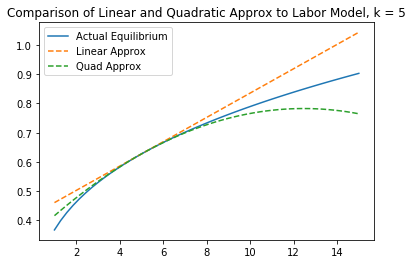
\includegraphics[scale = 0.5]{figP1}
		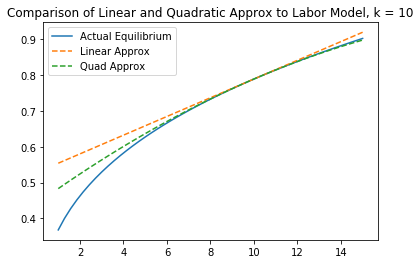
\includegraphics[scale = 0.5]{figP2}
	\end{figure}
	
	\newpage
	\subsection*{Exercise 3}
	We have the function $F(y,x) = (x^{.35} + .9x - y)^{-2.5} - .95(y^{.35} + .9y)^{-2.5} = 0$. We can simplify this as follows:
	\begin{align*}
	x^{.35} + .9x - y - .95^{-1/2.5}(y^{.35} + .9y) = 0
	\end{align*}
	Now we can use our formulas to compute $G_x(x_0)$, $G_{xx}(x_0)$, and $G_{xxx}(x_0)$. 
	\begin{align*}
	G_{x}(x_0) &= - \frac{F_x}{F_y} \\
	G_{xx}(x_0) &= - \frac{F_{yy} G_x^2 + 2 F_{xy} + F_{xx} }{F_{y}} \\
	G_{xxx}(x_0) &= - \frac{F_{yyy}G_x^2 + 3 F_{yyx} G_x^2 + 3 F_{yy} G_x G_{xx} + 3 F{xy} G_{xx} + 3 F_{yxx} G_x + F_{xxx} }{F_y}
	\end{align*}
	
	To facilitate coding this, we can solve each of these partial derivatives for the function.
	\begin{align*}
	F_{x} &= .35 x^{-.65} + .9 \\
	F_{y} &= -1 - .95^{-.4}(.35 y^{-.65} + .9) \\
	F_{xx} &= .35(-.65) x^{-1.65} \\
	F_{yy} &= .95^{-.4}(.35(-.65)y^{-1.65}) \\
	F_{xy} &= 0 \\
	F_{xyx} &= F_{xxy} = F_{yyx} = 0 \\
	F_{xxx} &= .35(-.65)(-1.65) x^{-2.65} \\
	F_{yyy} &= .95^{-.4}(.35(-.65)(-1.65)y^{-2.65})
	\end{align*}
	
	We can perform this computation in python, including printing the functional form of our polynomial. We note that the actually equilibrium value appears to be linear over the range we are considering , and so all of our approximations appear to be accurate. This can also be seen from the small coefficients on the quadratic and cubic terms in our functional form.
	
	\begin{figure}[!h]
		\centering
		\caption{Comparison of Solutions to F(y,x)}
		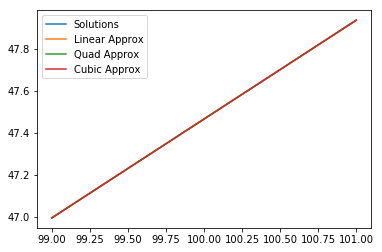
\includegraphics[scale = 0.5]{figP3}
	\end{figure}
	
	\newpage
	\subsection*{Exercise 4}
	We begin by taking the first derivatives of our Euler Equation in Section 3. Note that we have $y = x(x) = K_{t+2}$, $x = x(u) = K_{t+1}$, $u = K_t$.
	\begin{align*}
	F_y &= - \beta \alpha \frac{K_{t+1}^{\alpha -1}}{(K_{t+1}^{\alpha} - K_{t+2})^2} \\
	F_x &= \frac{1}{(K_{t}^\alpha - K_{t+1})^2} - \beta \alpha \frac{ (\alpha -1) K_{t+1}^{\alpha - 2} (K_{t+1}^{\alpha} - K_{t+2}) -\alpha K_{t+1}^{2(\alpha -1)}}{(K_{t+1}^{\alpha} - K_{t+2})^2} \\
	F_u &= - \frac{\alpha K_t^{\alpha -1}}{(K_t^{\alpha} - K_{t+1})^2} 
	\end{align*}
	
	Now we note that we can find $H_X$ by solving the quadratic equation $F_y H_X^2 + F_x H_X + H_X = 0$. 

	To find $H_{XX}$, we would need to analytically find the second derivatives.
	\begin{align*}
	F_{yu} &= 0 \\
	F_{yx} &= - \beta \alpha \frac{(\alpha -1)K_{t+1}^{\alpha -2} (K_{t+1}^{\alpha} - K_{t+2})^2 - 2 \alpha K_{t+1}^{2(\alpha -1)} (K_{t+1}^{\alpha} - K_{t+2}) }{(K_{t+1}^{\alpha} - K_{t+2})^4} \\
	F_{yy} &= - 2 \beta \alpha \frac{K_{t+1}^{\alpha -1}}{(K_{t+1}^{\alpha} - K_{t+2})^3} \\
	F_{xx} &= \frac{2}{(K_t^{\alpha} - K_{t+1})^3} - \\
	& \beta \alpha \frac{((\alpha -1)(2\alpha -2) K_{t+1}^{2\alpha -3} - (\alpha -1)(\alpha -2) K_{t+1}^{\alpha -3} K_{t+2} - \alpha (2(\alpha -1)) K_{t+1}^{2\alpha -3})(K_{t+1}^{\alpha} - K_{t+2})^2 }{(K_{t+1}^{\alpha} - K_{t+2})^4} - \\
	& \beta \alpha \frac{- 2\alpha K_{t+1}^{\alpha -1} ((\alpha -1)K_{t+1}^{\alpha -2}(K_{t+1}^{\alpha} - K_{t+2}) - \alpha _{t+1}^{2(\alpha -1)})(K_{t+1}^{\alpha} - K_{t+2})}{(K_{t+1}^{\alpha} - K_{t+2})^4}\\
	F_{uu} &=  - \frac{\alpha(\alpha -1) K_t^{\alpha -2} (K_t^{\alpha} - K_{t+1})^2 - 2 \alpha^2 K_{t}^{2(\alpha -1)}(K_{t}^{\alpha} - K_{t+1})}{(K_t^{\alpha} - K_{t+1})^4} \\
	F_{ux} &= - 2 \frac{\alpha K_{t}^{\alpha -1}}{(K_t^\alpha - K_{t+1})^3}
	\end{align*}
	
	Now we can input these analytical functions into python to obtain $H_X$ and $H_{XX}$. 
	
	\begin{figure}[!h]
		\centering
		\caption{Solutions to Brock and Mirman Model}
		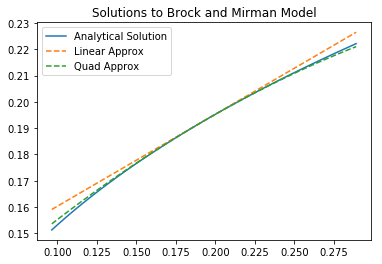
\includegraphics[scale=0.7]{figP4}
	\end{figure}
	
	\newpage
	\subsection*{Exercise 5}
	We can also implement a quadratic approximation using the perturbation method to our stochastic Brock and Mirman model. We implement this in the attached Python notebook.
	
	Some key points to note is that for this model, $n_X = n_Z = 1$, and $n_Y = 0$. This means that all of our block matrices are really just single values, which simplifies calculations and syntax somewhat. 
	
	In addition, we also note that the single shock implies that $\Omega = 1$, and $v = \sigma = 0.02$ as specified. 
	
	Our policy function from this approximation is shown below.
	\begin{figure}[!h]
		\centering
		\caption{Plot of Quadratic Approximation}
		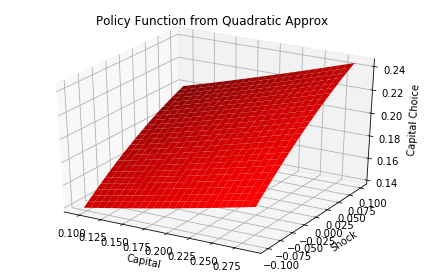
\includegraphics[scale = 0.5]{figP5}
	\end{figure}
\end{document}